\documentclass{sigchi-ext}
% Please be sure that you have the dependencies (i.e., additional
% LaTeX packages) to compile this example.
\usepackage[T1]{fontenc}
\usepackage{textcomp}
\usepackage[scaled=.92]{helvet} % for proper fonts
\usepackage{graphicx} % for EPS use the graphics package instead
\usepackage{balance}  % for useful for balancing the last columns
\usepackage{booktabs} % for pretty table rules
\usepackage{ccicons}  % for Creative Commons citation icons
\usepackage{ragged2e} % for tighter hyphenation

% Some optional stuff you might like/need.
% \usepackage{marginnote} 
% \usepackage[shortlabels]{enumitem}
% \usepackage{paralist}
% \usepackage[utf8]{inputenc} % for a UTF8 editor only

%% EXAMPLE BEGIN -- HOW TO OVERRIDE THE DEFAULT COPYRIGHT STRIP --
% \copyrightinfo{Permission to make digital or hard copies of all or
% part of this work for personal or classroom use is granted without
% fee provided that copies are not made or distributed for profit or
% commercial advantage and that copies bear this notice and the full
% citation on the first page. Copyrights for components of this work
% owned by others than ACM must be honored. Abstracting with credit is
% permitted. To copy otherwise, or republish, to post on servers or to
% redistribute to lists, requires prior specific permission and/or a
% fee. Request permissions from permissions@acm.org.\\
% {\emph{CHI'14}}, April 26--May 1, 2014, Toronto, Canada. \\
% Copyright \copyright~2014 ACM ISBN/14/04...\$15.00. \\
% DOI string from ACM form confirmation}
%% EXAMPLE END

% Paper metadata (use plain text, for PDF inclusion and later
% re-using, if desired).  Use \emtpyauthor when submitting for review
% so you remain anonymous.
\def\plaintitle{SIGCHI Extended Abstracts Sample File: Note Initial
  Caps} \def\plainauthor{First Author, Second Author, Third Author,
  Fourth Author, Fifth Author, Sixth Author}
\def\emptyauthor{}
\def\plainkeywords{Authors' choice; of terms; separated; by
  semicolons; include commas, within terms only; required.}
\def\plaingeneralterms{Documentation, Standardization}

\title{SIGCHI Extended Abstracts Sample File: \underline{N}ote
  \underline{I}nitial \underline{C}aps}

\numberofauthors{6}
% Notice how author names are alternately typesetted to appear ordered
% in 2-column format; i.e., the first 4 autors on the first column and
% the other 4 auhors on the second column. Actually, it's up to you to
% strictly adhere to this author notation.
\author{%
  \alignauthor{%
    \textbf{First Author}\\
    \affaddr{University of Author} \\
    \affaddr{Authortown, CA 94022, USA} \\
    \email{author1@anotherco.edu} }\alignauthor{%
    \textbf{Fifth Author}\\
    \affaddr{YetAuthorCo, Inc.}\\
    \affaddr{Authortown, BC V6M 22P Canada}\\
    \email{author5@anotherco.com} } \vfil \alignauthor{%
    \textbf{Second Author}\\
    \affaddr{VP, Authoring}\\
    \affaddr{Authorship Holdings, Ltd.}\\
    \affaddr{Awdur SA22 8PP, UK}\\
    \email{author2@author.ac.uk} }\alignauthor{%
    \textbf{Sixth Author}\\
    \affaddr{Universit\'e de Auteur-Sud}\\
    \affaddr{40222 Auteur France}\\
    \email{author6@author.fr} } \vfil \alignauthor{%
    \textbf{Third Author}\\
    \textbf{Fourth Author}\\    
    \affaddr{L\={e}khaka Interaction Labs}\\
    \affaddr{Bengaluru 560 080, India}\\
    \email{author3@anotherco.com} \\
    \email{author4@hchi.anotherco.com} }\alignauthor{%
    \textbf{Seventh Author}\\
    \affaddr{Department of Skrywer}\\
    \affaddr{University of Umbhali}\\
    \affaddr{Cape Town, South Africa}\\
    \email{author7@umbhaliu.ac.za} } }

% Make sure hyperref comes last of your loaded packages, to give it a
% fighting chance of not being over-written, since its job is to
% redefine many LaTeX commands.
\definecolor{linkColor}{RGB}{6,125,233}
\hypersetup{%
  pdftitle={\plaintitle},
%  pdfauthor={\plainauthor},
  pdfauthor={\emptyauthor},
  pdfkeywords={\plainkeywords},
  bookmarksnumbered,
  pdfstartview={FitH},
  colorlinks,
  citecolor=black,
  filecolor=black,
  linkcolor=black,
  urlcolor=linkColor,
  breaklinks=true,
}

% \reversemarginpar%

\begin{document}

%% For the camera ready, use the commands provided by the ACM in the Permission Release Form.
%\CopyrightYear{2007}
%\setcopyright{rightsretained}
%\conferenceinfo{WOODSTOCK}{'97 El Paso, Texas USA}
%\isbn{0-12345-67-8/90/01}
%\doi{http://dx.doi.org/10.1145/2858036.2858119}
%% Then override the default copyright message with the \acmcopyright command.
%\copyrightinfo{\acmcopyright}

\maketitle

% Uncomment to disable hyphenation (not recommended)
% https://twitter.com/anjirokhan/status/546046683331973120
\RaggedRight{} 

% Do not change the page size or page settings.
\begin{abstract}
  UPDATED---\today. This sample paper describes the formatting
  requirements for SIGCHI Extended Abstract Format, and this sample
  file offers recommendations on writing for the worldwide SIGCHI
  readership. Please review this document even if you have submitted
  to SIGCHI conferences before, as some format details have changed
  relative to previous years. Abstracts should be about 150
  words. Required.
\end{abstract}

\keywords{\plainkeywords}

\category{H.5.m}{Information interfaces and presentation (e.g.,
  HCI)}{Miscellaneous}\category{See}{\url{http://acm.org/about/class/1998/}}{for
  full list of ACM classifiers. This section is required.}

\section{Introduction}
This format is to be used for submissions that are published in the
conference publications. We wish to give this volume a consistent,
high-quality appearance. We therefore ask that authors follow some
simple guidelines. In essence, you should format your paper exactly
like this document. The easiest way to do this is to replace the
content with your own material.

\section{ACM Copyrights \& Permission}
Accepted extended abstracts and papers will be distributed in the
Conference Publications. They will also be placed in the ACM Digital
Library, where they will remain accessible to thousands of researchers
and practitioners worldwide. To view the ACM's copyright and
permissions policy, see:
\url{http://www.acm.org/publications/policies/copyright_policy}.

\marginpar{%
  \vspace{-45pt} \fbox{%
    \begin{minipage}{0.925\marginparwidth}
      \textbf{Good Utilization of the Side Bar} \\
      \vspace{1pc} \textbf{Preparation:} Do not change the margin
      dimensions and do not flow the margin text to the
      next page. \\
      \vspace{1pc} \textbf{Materials:} The margin box must not intrude
      or overflow into the header or the footer, or the gutter space
      between the margin paragraph and the main left column. The text
      in this text box should remain the same size as the body
      text. Use the \texttt{{\textbackslash}vspace{}} command to set
      the margin
      note's position. \\
      \vspace{1pc} \textbf{Images \& Figures:} Practically anything
      can be put in the margin if it fits. Use the
      \texttt{{\textbackslash}marginparwidth} constant to set the
      width of the figure, table, minipage, or whatever you are trying
      to fit in this skinny space.
    \end{minipage}}\label{sec:sidebar} }

\section{Page Size}
All SIGCHI submissions should be US letter (8.5 $\times$ 11
inches). US Letter is the standard option used by this \LaTeX\
template.

\section{Text Formatting}
Please use an 8.5-point Verdana font, or other sans serifs font as
close as possible in appearance to Verdana in which these guidelines
have been set. Arial 9-point font is a reasonable substitute for
Verdana as it has a similar x-height. Please use serif or
non-proportional fonts only for special purposes, such as
distinguishing \texttt{source code} text.

\subsubsection{Text styles}
The \LaTeX\ template facilitates text formatting for normal (for body
text); heading 1, heading 2, heading 3; bullet list; numbered list;
caption; annotation (for notes in the narrow left margin); and
references (for bibliographic entries). Additionally, here is an
example of footnoted\footnote{Use footnotes sparingly, if at all.}
text. As stated in the footnote, footnotes should rarely be used.

\begin{figure}
  
\includegraphics[width=0.9\columnwidth]{figures/sigchi-logo}
  \caption{Insert a caption below each figure.}~\label{fig:sample}
\end{figure}

\subsection{Language, style, and content}
The written and spoken language of SIGCHI is English. Spelling and
punctuation may use any dialect of English (e.g., British, Canadian,
US, etc.) provided this is done consistently. Hyphenation is
optional. To ensure suitability for an international audience, please
pay attention to the following:

\begin{table}
  \centering
  \begin{tabular}{l r r r}
    % \toprule
    & & \multicolumn{2}{c}{\small{\textbf{Test Conditions}}} \\
    \cmidrule(r){3-4}
    {\small\textit{Name}}
    & {\small \textit{First}}
      & {\small \textit{Second}}
    & {\small \textit{Final}} \\
    \midrule
    Marsden & 223.0 & 44 & 432,321 \\
    Nass & 22.2 & 16 & 234,333 \\
    Borriello & 22.9 & 11 & 93,123 \\
    Karat & 34.9 & 2200 & 103,322 \\
    % \bottomrule
  \end{tabular}
  \caption{Table captions should be placed below the table. We
    recommend table lines be 1 point, 25\% black. Minimize use of
    table grid lines.}~\label{tab:table1}
\end{table}

\begin{itemize}\compresslist%
\item Write in a straightforward style. Use simple sentence
  structure. Try to avoid long sentences and complex sentence
  structures. Use semicolons carefully.
\item Use common and basic vocabulary (e.g., use the word ``unusual''
  rather than the word ``arcane'').
\item Briefly define or explain all technical terms. The terminology
  common to your practice/discipline may be different in other design
  practices/disciplines.
\item Spell out all acronyms the first time they are used in your
  text. For example, ``World Wide Web (WWW)''.
\item Explain local references (e.g., not everyone knows all city
  names in a particular country).
\item Explain ``insider'' comments. Ensure that your whole audience
  understands any reference whose meaning you do not describe (e.g.,
  do not assume that everyone has used a Macintosh or a particular
  application).
\item Explain colloquial language and puns. Understanding phrases like
  ``red herring'' requires a cultural knowledge of English. Humor and
  irony are difficult to translate.
\item Use unambiguous forms for culturally localized concepts, such as
  times, dates, currencies, and numbers (e.g., ``1-5- 97'' or
  ``5/1/97'' may mean 5 January or 1 May, and ``seven o'clock'' may
  mean 7:00 am or 19:00). For currencies, indicate equivalences:
  ``Participants were paid {\fontfamily{txr}\selectfont \textwon}
  25,000, or roughly US \$22.''
\item Be careful with the use of gender-specific pronouns (he, she)
  and other gender-specific words (chairman, manpower,
  man-months). Use inclusive language (e.g., she or he, they, chair,
  staff, staff-hours, person-years) that is gender-neutral. If
  necessary, you may be able to use ``he'' and ``she'' in alternating
  sentences, so that the two genders occur equally
  often~\cite{Schwartz:1995:GBF}.
\item If possible, use the full (extended) alphabetic character set
  for names of persons, institutions, and places (e.g.,
  Gr{\o}nb{\ae}k, Lafreni\'ere, S\'anchez, Nguy{\~{\^{e}}}n,
  Universit{\"a}t, Wei{\ss}enbach, Z{\"u}llighoven, \r{A}rhus, etc.).
  These characters are already included in most versions and variants
  of Times, Helvetica, and Arial fonts.
\end{itemize}

% \begin{figure}
%   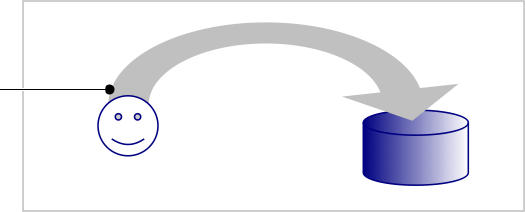
\includegraphics[width=.9\columnwidth]{figures/ea-figure2}
%   \caption{If your figure has a light background, you can set its
%     outline to light gray, like this, to make a box around
%     it.}\label{fig:bats}
% \end{figure}

\begin{marginfigure}[-35pc]
  \begin{minipage}{\marginparwidth}
    \centering
    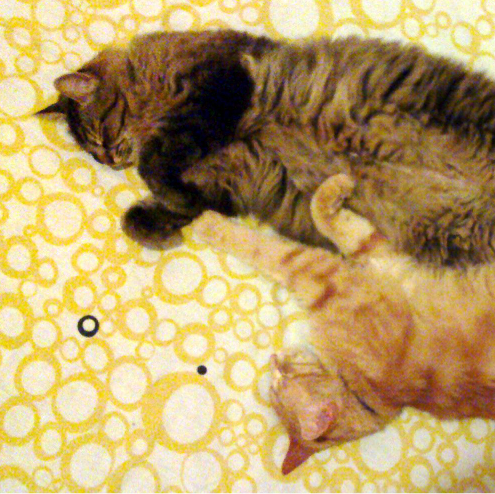
\includegraphics[width=0.9\marginparwidth]{figures/cats}
    \caption{In this image, the cats are tessellated within a square
      frame. Images should also have captions and be within the
      boundaries of the sidebar on page~\pageref{sec:sidebar}. Photo:
      \cczero~jofish on Flickr.}~\label{fig:marginfig}
  \end{minipage}
\end{marginfigure}

\section{Figures}
The examples on this and following pages should help you get a feel
for how screen-shots and other figures should be placed in the
template. Your document may use color figures (see
Figures~\ref{fig:sample}), which are included in the page limit; the
figures must be usable when printed in black and white. You can use
the \texttt{\marginpar} command to insert figures in the (left) margin
of the document (see Figure~\ref{fig:marginfig}). Finally, be sure to
make images large enough so the important details are legible and
clear (see Figure~\ref{fig:cats}).

\section{Tables}
You man use tables inline with the text (see Table~\ref{tab:table1})
or within the margin as shown in Table~\ref{tab:table2}. Try to
minimize the use of lines (especially vertical lines). \LaTeX\ will
set the table font and captions sizes correctly; the latter must
remain unchanged.

\section{Accessibility}
The Executive Council of SIGCHI has committed to making SIGCHI
conferences more inclusive for researchers, practitioners, and
educators with disabilities. As a part of this goal, the all authors
are asked to work on improving the accessibility of their
submissions. Specifically, we encourage authors to carry out the
following five steps:
\begin{itemize}\compresslist%
\item Add alternative text to all figures
\item Mark table headings
\item Generate a tagged PDF
\item Verify the default language
\item Set the tab order to ``Use Document Structure''
\end{itemize}

For links to instructions and resources, please see:
\url{http://chi2016.acm.org/accessibility}

Unfortunately good tools do not yet exist to create tagged PDF files
from Latex. \LaTeX\ users will need to carry out all of the above
steps in the PDF directly using Adobe Acrobat, after the PDF has been
generated.

For more information and links to instructions and resources, please
see:
\url{http://chi2016.acm.org/accessibility}.

\begin{figure*}
  \centering
  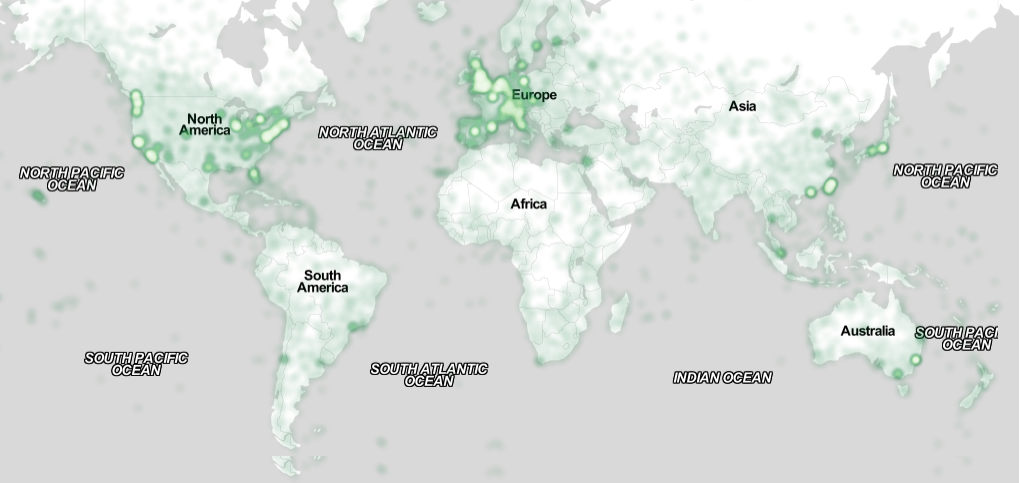
\includegraphics[width=1.3\columnwidth]{figures/map}
  \caption{In this image, the map maximizes use of space. You can make
    figures as wide as you need, up to a maximum of the full width of
    both columns. Note that \LaTeX\ tends to render large figures on a
    dedicated page. Image: \ccbynd~ayman on Flickr.}~\label{fig:cats}
\end{figure*}

\section{Producing and Testing PDF Files}
We recommend that you produce a PDF version of your submission well
before the final deadline. Your PDF file must be ACM DL Compliant and
meet stated requirements,
\url{http://www.sheridanprinting.com/sigchi/ACM-SIG-distilling-settings.htm}.

\marginpar{\vspace{-23pc}So long as you don't type outside the right
  margin or bleed into the gutter, it's okay to put annotations over
  here on the left, too; this annotation is near Hawaii. You'll have
  to manually align the margin paragraphs to your \LaTeX\ floats using
  the \texttt{{\textbackslash}vspace{}} command.}

\begin{margintable}[1pc]
  \begin{minipage}{\marginparwidth}
    \centering
    \begin{tabular}{r r l}
      & {\small \textbf{First}}
      & {\small \textbf{Location}} \\
      \toprule
      Child & 22.5 & Melbourne \\
      Adult & 22.0 & Bogot\'a \\
      \midrule
      Gene & 22.0 & Palo Alto \\
      John & 34.5 & Minneapolis \\
      \bottomrule
    \end{tabular}
    \caption{A simple narrow table in the left margin
      space.}~\label{tab:table2}
  \end{minipage}
\end{margintable}
Test your PDF file by viewing or printing it with the same software we
will use when we receive it, Adobe Acrobat Reader Version 10. This is
widely available at no cost. Note that most
reviewers will use a North American/European version of Acrobat
reader, so please check your PDF accordingly.

\section{Acknowledgements}
We thank all the volunteers, publications support, staff, and authors
who wrote and provided helpful comments on previous versions of this
document. As well authors 1, 2, and 3 gratefully acknowledge the grant
from NSF (\#1234--2222--ABC). Author 4 for example may want to
acknowledge a supervisor/manager from their original employer. This
whole paragraph is just for example. Some of the references cited in
this paper are included for illustrative purposes only.

\section{References Format}
Your references should be published materials accessible to the
public. Internal technical reports may be cited only if they are
easily accessible and may be obtained by any reader for a nominal
fee. Proprietary information may not be cited. Private communications
should be acknowledged in the main text, not referenced (e.g.,
[Golovchinsky, personal communication]). References must be the same
font size as other body text. References should be in alphabetical
order by last name of first author. Use a numbered list of references
at the end of the article, ordered alphabetically by last name of
first author, and referenced by numbers in brackets. For papers from
conference proceedings, include the title of the paper and the name of
the conference. Do not include the location of the conference or the
exact date; do include the page numbers if available. 

References should be in ACM citation format:
\url{http://www.acm.org/publications/submissions/latex_style}.  This
includes citations to Internet
resources~\cite{CHINOSAUR:venue,cavender:writing,psy:gangnam}
according to ACM format, although it is often appropriate to include
URLs directly in the text, as above. Example reference formatting for
individual journal articles~\cite{ethics}, articles in conference
proceedings~\cite{Klemmer:2002:WSC:503376.503378},
books~\cite{Schwartz:1995:GBF}, theses~\cite{sutherland:sketchpad},
book chapters~\cite{winner:politics}, an entire journal
issue~\cite{kaye:puc},
websites~\cite{acm_categories,cavender:writing},
tweets~\cite{CHINOSAUR:venue}, patents~\cite{heilig:sensorama}, 
games~\cite{supermetroid:snes}, and
online videos~\cite{psy:gangnam} is given here.  See the examples of
citations at the end of this document and in the accompanying
\texttt{BibTeX} document. This formatting is a edited version of the
format automatically generated by the ACM Digital Library
(\url{http://dl.acm.org}) as ``ACM Ref''. DOI and/or URL links are
optional but encouraged as are full first names. Note that the
Hyperlink style used throughout this document uses blue links;
however, URLs in the references section may optionally appear in
black.

\balance{} 

\bibliographystyle{SIGCHI-Reference-Format}
\bibliography{sample}

\end{document}

%%% Local Variables:
%%% mode: latex
%%% TeX-master: t
%%% End:
